\documentclass{beamer}
 
\usepackage[utf8]{inputenc}
\usepackage{amsmath,amsthm,amssymb}
\usepackage{graphicx}
\usepackage{listings}
\usepackage{color}
\usepackage[document]{ragged2e}
\usepackage[font=small,labelfont=bf]{caption}
\usepackage{bussproofs}
\usepackage{syntax}
\usepackage{mathtools}
\usepackage{tikz-cd}
\newcommand*\pipenotdiv{\,\nmid\,}
\newcommand*\pipediv{\,|\,}
\usetheme{Madrid}

\lstset{
  frame=none,
  xleftmargin=2pt,
  stepnumber=1,
  numbers=left,
  numbersep=5pt,
  numberstyle=\ttfamily\tiny\color[gray]{0.3},
  belowcaptionskip=\bigskipamount,
  captionpos=b,
  escapeinside={*'}{'*},
  language=haskell,
  tabsize=2,
  emphstyle={\bf},
  commentstyle=\it,
  stringstyle=\mdseries\rmfamily,
  showspaces=false,
  keywordstyle=\bfseries\rmfamily,
  columns=flexible,
  basicstyle=\small\sffamily,
  showstringspaces=false,
  morecomment=[l]\%,
}

\DeclarePairedDelimiter{\norm}{\lVert}{\rVert}

 
%Information to be included in the title page:
\title[Fundamentals of Lattice-Based Crypto]{Fun with Lattices! \\ (a.k.a Fundamentals of Lattice-Based Cryptography)}
\author{Jose Cardona}
\institute{OQuant}
\date[LC 2019]{LambdaConf 2019}
%\graphicspath{{/home/jm0x5c/Documents/presentations/LC/images/}}

\newcommand{\lat}{\mathcal{L}}
\newcommand{\rat}{\mathbb{R}}
\newcommand{\zee}{\mathbb{Z}}

 
\begin{document}
 
\frame{\titlepage}

\author[Jose, Cardona] % (optional, for multiple authors)
{}

\begin{frame}
\frametitle{Why lattices?}

Lattices are incredible mathematical objects with applications outside of the ones we'll view today!

\begin{itemize}
\item In Number theory, lattices have been used to test various conjectures (See: disproof of Merten's conjecture)
\item In Complexity Theory, lattices have a special place in that for certain problems, finding a solution in a "random lattice" is as hard as a solution in worst case complexity! (Ajitai)
\item In Error Correcting Codes, Lattices + The Sphere packing problem (Which also uses lattices) are used for ECC construction.
\end{itemize}

Today, we tackle the application that interests me the most: Lattices used to construct Cryptosystems!

\end{frame}

\begin{frame}
\frametitle{Table Of Contents}

\begin{enumerate}
\item Vector Spaces
\item Lattices
\item GGH
\item Convolution Polynomials and NTRU
\item (BONUS) Lattice-Reductions (LLL)
\item (BONUS) Short Integer Solutions
\item (BONUS) LWE
\end{enumerate}

\end{frame}

\begin{frame}
\frametitle{Our Goal Today}
\begin{center}
\includegraphics[scale=1]{House-Foundation.jpg}
\end{center}

\end{frame}

\begin{frame}
\frametitle{}

\begin{enumerate}
\item \textbf{Vector Spaces}
\item Lattices
\item GGH
\item Convolution Polynomials and NTRU
\item (BONUS) Lattice-Reductions (LLL)
\item (BONUS) Short Integer Solutions
\item (BONUS) LWE
\end{enumerate}

\end{frame}

\begin{frame}
\frametitle{Vector spaces}

A vector space $V$ over some field $F$ is an abelian group with a \textit{scalar product} $\forall \alpha \in F, \forall v \in V: \alpha v$ defined, that satisfies the following axioms:

\begin{itemize}
\item $\forall \alpha, \beta \in F,\forall v\in V : \alpha (\beta v) = (\alpha \beta) v$
\item $\forall \alpha, \beta \in F,\forall v\in V : (\alpha + \beta) v = \alpha v + \beta v$
\item $\forall \alpha, \beta \in F,\forall v\in V : \alpha (u+v) = \alpha u + \alpha v$		
\item $\forall v \in V : 1_{F}v = v$		
\end{itemize}

Such that 

\[ \forall \alpha, \beta \in F, \forall u, v \in V : \alpha u + \beta v \in V \]

Vector spaces are more general than how we use them (and can be generalized even more by modules), but in this presentation, the group we will be concerned with will be vectors in $\mathbb{R}^n$ for some $n \in \mathbb{N}$

\end{frame}

\begin{frame}
\frametitle{Vector spaces}
A linear combination of some set of vectors $v_1, v_2,..,v_k \in V$ is any vector of the form

\[ u = \alpha_1 v_1 + \alpha_2 v_2 + .. + \alpha_k v_k \text{ with } \alpha_1,..,\alpha_k \in F\]

The set of all linear combinations of the above is called the \textbf{span} of $v_1, ..., v_k$.	

A set of vectors is linearly independent if for the above, $ \alpha_1 v_1 + \alpha_2 v_2 + .. + \alpha_k v_k = 0$ implies $a_1 = a_2 = ... = a_k = 0$
\end{frame}

\begin{frame}
\frametitle{Vector spaces}
A \textbf{basis} for a vector space V is a set of linearly independent vectors

$v_1,..., v_n \in V$  that span $V$, such a way that every $w \in V$ is written as a \textit{unique} linear combination (in other words, unique combination of coefficients). Such a basis is said to have \textbf{dimension} (or dim) $n$.

Let $V \subset R^m$ be a vector space. Then:
\begin{itemize}
\item There exists a basis for $V$
\item Any two basis for V have the same number of elements.
\item The dimension of the basis cannot be larger than the dimension of the coordinate space (Meaning for basis of dimension n and $R^m$, $n <= m$).
\end{itemize}



\end{frame}


\begin{frame}
\frametitle{Vector spaces}
\underline{\textbf{Defn:}} The \textbf{dot product} of two vectors $v = (v_1, v_2, .., v_n)$ and $u = (u_1, u_2,...,u_n)$ is defined by the quantity:

\[ u \cdot v = \sum_{i=1}^n v_i u_i \]

\underline{\textbf{Defn:}} The length or Euclidean norm (or \textit{length}) of some vector $v = (v_1, v_2, .., v_n)$ is the quantity 

\[ \norm{v} = \sqrt{v_1^2+v_2^2+..+v_n^2} \]

The dot product and the Euclidean norm share a relationship via:

\[ v \cdot v = \norm{v}^2 \]

\end{frame}

\begin{frame}
\frametitle{Vector spaces}
\underline{\textbf{Defn}} (Cauchy-Schwarz inequality): For some vectors $v$, $w \in V \subset R^n$, 

\[ |v \cdot w | \leq \norm{v}\norm{w} \]

\underline{\textbf{Defn}} A basis $B$ is said to be \textbf{orthogonal} if for all $v_i, v_j \in B$ with $i \neq j$, $1 \leq i < j \leq n$ we have:

\[ v_i \cdot v_j = 0 \]

Said basis is \textit{orthonormal} if for any $v_i \in B$, $\norm{v_i} = 1$.

\end{frame} 

\begin{frame}
\begin{enumerate}
\item Vector Spaces
\item \textbf{Lattices}
\item GGH
\item Convolution Polynomials and NTRU
\item (BONUS) Lattice-Reductions (LLL)
\item (BONUS) Short Integer Solutions
\item (BONUS) LWE
\end{enumerate}
\end{frame}

\begin{frame}
\frametitle{Lattices}

Lattices, geometrically, are a set of points in n-dimensional Euclidean space that exhibit a periodic structure, the easiest of which to envision is, for example, a grid-like structure in two-dimensional space.

\begin{center}
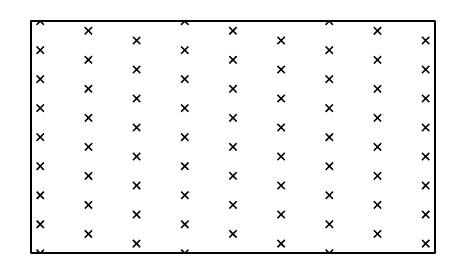
\includegraphics[scale=0.5]{Lattice-in-r2.jpeg}
\end{center}



\end{frame}

\begin{frame}
\frametitle{Lattices}
Let $B$ be a set of linearly independent vectors $B = {b_1, b_2, .., b_n}$ of dimension $n$.

The lattice $\mathcal{L}(b_1, b_2, .., b_n)$ 	is the discrete linear combinator of vectors spanned by the basis with integer coefficients, or:

\[ \mathcal{L}(b_1, b_2,..., b_n) = \big\{ \sum_{i=1}^n a_i b_i | a_i \in \mathbb{Z} \big\} \]

By \textit{discrete}, it means that there exists some $\epsilon > 0$ such that the distance between any two lattice vectors is at least $\epsilon$.

Geometrically, this corresponds to drawing an n-dimensional ball centered around some vector coordinate in $R^n$. 

It turns out that a subset of $R^m$ is a lattice if and only if it is a discrete, additive subgroup (We will come back to the proof of this!).

\end{frame}

\begin{frame}
\frametitle{Lattices}

For any lattice of dimension $n$ with basis $b_1, ..., b_n$, we define the \textit{Fundamental Parallelepiped} $\mathcal{F}$ as the set

\[ \mathcal{F}(b_1,...,b_n) =  \bigg\{ \sum x_i b_i  \, | \,  x_i \in R^n, 1 \leq i \leq n, 0 \leq x_i < 1  \bigg\} \]

\begin{center}
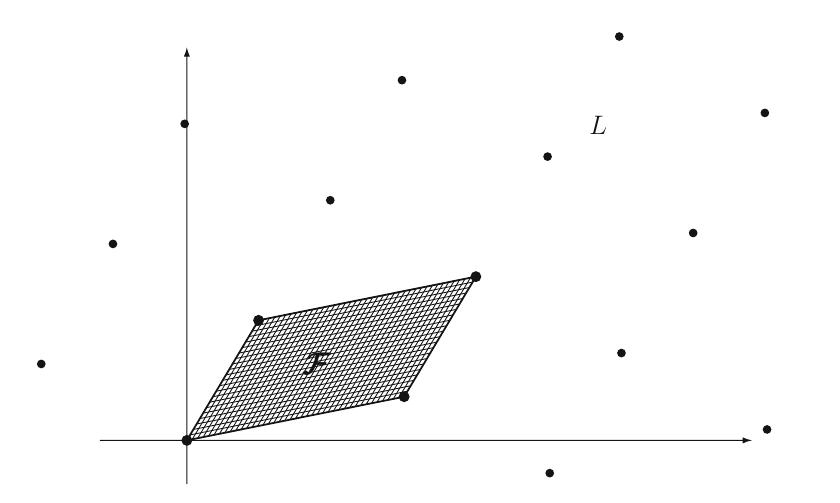
\includegraphics[scale=0.3]{Fundamental-para.png}
\end{center}

\end{frame}

\begin{frame}
\frametitle{Lattices}
Fundamental Parallelepipeds are interesting to us since, even by naiive inspection, we can observe a few things:
\begin{itemize}
\item Fundamental Parallelepipeds give us an "area" to work with when we want to describe how big are the "cells" that make up our n-dimensional lattice.
\item It almost looks like they "tile" our lattice.
\end{itemize}

Unrelated: Paralelepiped. I love that word.

\end{frame}

\begin{frame}
\frametitle{Lattices}
With these notions in hand, it turns out that the intuitions are actually correct! Fundamental Parallelepipeds in fact provide us with both a notion of tiling and "volume". We will start with the former.

\vspace{2em}

Proposition (L1): Let $L$ is a full rank lattice in $R^n$, $\mathcal{F}$ a F.P. for $L$. Then we can write every vector in $w \in R^n$ as:

\[ w = u + f, \text{  for some unique } u \in L, f \in \mathcal{F} \]

Equivalently, we can say for all $u \in L$, $u + F = \{ u + f \, | \, f \in \mathcal{F} \}$ forms a partition of $R^n$.

\end{frame}

\begin{frame}
\frametitle{Lattices}

We can observe the idea from the previous slide in $R^2$ as such:

\begin{center}
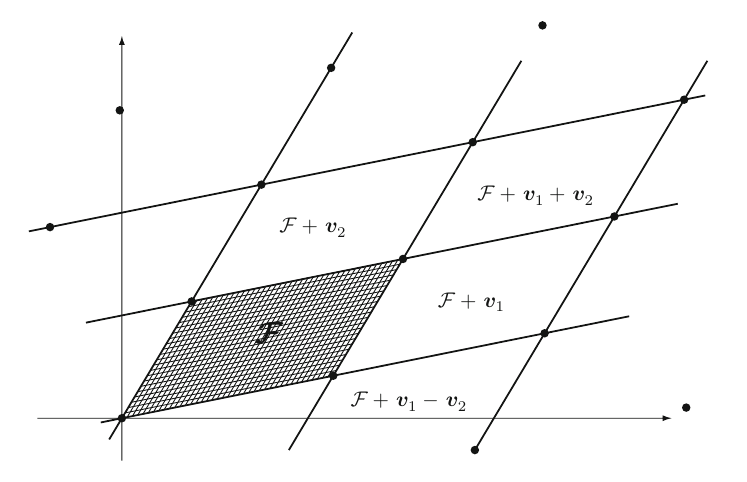
\includegraphics[scale=0.4]{Fundamental-para-span.png}
\end{center}

\end{frame}

\begin{frame}
\frametitle{Lattices}
\underline{\textit{Proof (L1)}}: For our full rank lattice $L$, let the basis of $L$ be $b_1,...,b_n$. We know since it is a full rank lattice, the basis also spans $R^n$.

Thus, every vector in $\mathbb{R}^n$ is of the form $a_1 b_1 + ...+ a_n b_n$ with $a_i \in \mathbb{R}$.

\vspace{1em}

We can also consider writing every $a_i$ in the form $a_i = \alpha_i + t_i$ where $\alpha_i \in \mathbb{Z}, t_i \in \mathbb{R}, 0 \leq t_i < 1$, which is an equivalent formulation.

\vspace{1em}

WLOG for any $a_i b_i$ we can transform it as:
\begin{align*}
a_i b_i &= (\alpha_i + t_i) b_i \\
 &= \alpha_i b_i + t_i b_i
\end{align*}

Where now $\alpha_i b_i$ is an element of $L$ and $t_i b_i$ is an element of $\mathcal{F}$.

\end{frame}

\begin{frame}
\frametitle{Lattices}
\underline{\textit{Proof (L1)}} (Cont): The only thing left now is to prove that each combination of unique representatives will yield a unique vector, which is quick.

\vspace{1em}

WLOG pick one representative $(\alpha_i + t_i) b_i$ and let us assume there is a pair $\alpha_i' + t_i'$ such that $(\alpha_i + t_i) b_i = (\alpha_i' + t_i') b_i$.

\vspace{1em}

Then we can algebraically cancel $b_i$ and rearrange to yield

\[ \alpha_i - \alpha_i' = t_i - t_i' \]

However, we know that $\alpha_i$ and $\alpha_i'$ are both integers, so their difference should yield an integer. Thus, the only way $t_i$ and $t_i'$ yield an integer is if $t_i = t_i'$, proving that our vector is unique.

\end{frame}


\begin{frame}
\frametitle{Lattices}

Another way to think about (Full rank) lattices is as a set generated by the linear transformation of an $nxn$ matrix $A$ composed of the basis vectors columnwise, and a vector $x$ in $\mathbb{Z}^n$ such that:

\[ B = \begin{bmatrix}
| & & | \\
b_1 & .. & b_n \\
| & & |
\end{bmatrix}
\]

And the lattice $\mathcal{L}(B)$ is now defined as

\[ \mathcal{L}(B) = \{ Bx | x \in \mathbb{Z}^n\} \]

This definition becomes immediately useful when we consider: when do two linearly independent subsets of $R^m$ generate the same lattice?

\end{frame}

\begin{frame}
\frametitle{Lattices}

As an example, let's use:

\[ 
B_1 = \begin{bmatrix}
1 && 0 \\
0 && 1
\end{bmatrix}, B_2 = \begin{bmatrix}
2 && 1 \\
1 && 1
\end{bmatrix}
\]

It turns out that both bases generate the same lattice, but how?

Moreover, the matrix:

\[
B_3 = \begin{bmatrix}
41 & 41 \\
9 & 8
\end{bmatrix}
\]

Also has column vectors spanning $\mathbb{R}^2$, but $\mathcal{L}(B_1) = \mathcal{L}(B_2) \neq 
\lat(B_3)$. Why?


\end{frame}

\begin{frame}
\frametitle{Lattices}

\underline{\textbf{Defn}} A matrix $U$ is unimodular if $det(U) = \pm 1$.

It turns out we relate any two bases $B_1, B_2 \in \mathbb{R}^{nxn}$, such that they generate the same Lattice, if an only if there exists a \textit{unimodular} matrix $U$ such that $B_1 = B_2U$ (L2):
\vspace{1em}

\underline{\textit{Proof}}(L1) $(\implies)$:

\vspace{1em}

Assume $\mathcal{L}(B_1) = \mathcal{L}(B_2)$. Then for each column vector $b_{1i}$ of $B_1$, we have $b_{1i} \in \lat(B_2)$. 

This implies that there exists some matrix $U$ such that $B_1 = B_2U$. Apply the same argument backwards to each $b_{2i}$ of $B_2$ and you get $B_2 = B_1V$ for some matrix $V$.


\end{frame}

\begin{frame}
\frametitle{Lattices}
Thus we can, via simple algebraic substitution:
\begin{align*}
B_1 &= B_2U \\
B_1 &= (B_1V)U &&\text{ \textless substitution on previous slide.\textgreater}\\
B_1 &= B_1(VU) &&\text{ \textless matrix multiplication commutativity \textgreater} \\
I &= VU &&\text{ \textless left cancellation \textgreater}
\end{align*}

(Note: Left cancellation works on $B_1$ due to having linearly independent column vectors, thus it has an inverse).

Thus $VU$ are matrix inverses of each other, so we have $det(I) = det(VU) = 1$, which means $det(I) = det(V)det(U)$.
However given both are integer matrices, the only way this results to 1 is if the determinant of each is $\pm 1$.

We will do the converse together.

\end{frame}


\begin{frame}
\frametitle{Lattices}
Now that we've proven that two bases generate the same lattice if they have a unimodular linear transformation, there's a connection to be made with this. 

\vspace{1em}

From Linear algebra (this one is easy to forget), we know that the determinant of a matrix refers to the signed volume of the n-dimensional parallelepiped (for our purposes, ignore the sign). So we can simply refer to $Vol(F) = |det(B)|$ for some base $B$ that generates a lattice. 

\vspace{1em}

It then connects the dots that the fundamental parallelepiped for some lattice $\lat(B)$ should have the same volume no matter your choice of basis, meaning that a unimodular matrix is the only way you would be able to preserve volume while changing basis!

\end{frame}

\begin{frame}
\frametitle{Lattices}
In the interests of cryptography, with lattices, we want to somehow create constructions that under some "priviledged information" we can use to manipulate information. 

With cryptographic constructions based on fields of discrete points, the diffie-hellman problem comes to mind..

With cryptographic constructions like RSA, we have the prime factoring problem.

For the foundations of lattice cryptography, there exists a similar few problems.

\end{frame}

\begin{frame}
\frametitle{Lattices}
\textbf{The Shortest Vector Problem} (SVP) deals with trying to minimize the euclidean norm $\norm{v}$.

\vspace{1em}

\textbf{The Closest Vector Problem}(CVP) deals with, for some vector $a \in \rat^n$, find the vector $b$ in the lattice $L$ that minimizes the euclidean norm $\norm{a-b}$.

From these two, arise many important variants, with two we will see:

\vspace{1em}

\textbf{Approximate SVP} (apprSVP): Don't just minimize Euclidean norm, find a vector $v$ that for some function $\phi(n)$ (with $n$ being the dimension of the lattice), we minimize
\[ \norm{v} \leq \phi(n) \norm{v_{shortest}} \]

\vspace{1em}

\textbf{Approximate CVP} (apprCVP): same as above except approximating the closest vector.

\end{frame}

\begin{frame}
\frametitle{Lattices}
An important metric is the shortest nonzero vector, which we can denote as $\lambda_1$. We can also think about $\lambda_1$, as a closed ball of radius $r$, which gives a space that only contains one point of the lattice (or equivalently, the lattice points inside the ball span a space of dimension 1).

\vspace{1em}

So for some Lattice L, we have:

\[ \lambda_1(L) = inf \{ r \, | \, dim(span(L \cap \overline{B}(0,r))) \geq 1 \} \]

It turns out this concept is easy to generalize, and thus we have \textit{successive minima}, defined by

\[ \lambda_i(L) = inf \{ r \, | \, dim(span(L \cap \overline{B}(0,r))) \geq i \} \]


\end{frame}

\begin{frame}
\frametitle{Lattices}

Successive minima might not be defined as a vector belonging to some lattice $L$, but due to the property of discreteness of lattices, it turns out that there's a correspondence between successive minima and progressively nth smallest vectors in $\rat^n$.

Successive minima give us a lower bound on the length of the shortest vector in $L$.

\vspace{1em}

Proposition: Let $B$ be the basis of some lattice $\lat(B)$ of rank $n$, and $\widetilde{B}$ it's Gram-Schmidt orthogonalization, then we have

\[ \lambda_1 \geq min_{i \leq n} \norm{\tilde{b_i}} > 0 \]

for some $\tilde{b_i}$ as a column vector of $\widetilde{B}$

\end{frame}

\begin{frame}
\frametitle{Lattices}
Proof: If we consider $x \in \zee^n$ to be an arbitrary non-zero integer, we can show $\norm{Bx} \geq min \norm{b_i}$. Pick the largest nonzero element of $x$, denoted as $x_j$ for an integer $j \in [1, n]$. If we take $(Bx) \cdot \tilde{b_j}$, we have:

\[ |(Bx) \cdot \tilde{b_j}| = |(\sum_{i=1}^j x_i b_i) \cdot \tilde{b_j}| \]


\end{frame}

\begin{frame}
\frametitle{Lattices}
But notice that for Gram-Schmidt orthogonalized matrices, not only are the column vectors are orthogonal basis, but forall $i < j$, $b_i \cdot \tilde{b_j} = 0$, so then we have

\begin{align*}
|(Bx) \cdot \tilde{b_j}| &= |(\sum_{i=1}^j x_i b_i) \cdot \tilde{b_j}| \\
 &= |(\sum_{i=1}^j x_i b_i \cdot \tilde{b_j})| && \text{ (distrib over addition)} \\
 &= |x_j (b_j \cdot \tilde{b_j})| && \text{(orthogonal for all i < j)} \\
 &= |x_j||(\tilde{b_j} \cdot \tilde{b_j})| && \text{equality of dot products} \\
 &= |x_j|\norm{\tilde{b_j}}^2
\end{align*} 

\end{frame}

\begin{frame}
\frametitle{Lattices}
From Cauchy-Schwartz we have: $|(Bx) \cdot \tilde{b_j}| \leq \norm{Bx} \norm{ \tilde{b_j}}$, so we can conclude that

\begin{align*}
\norm{Bx} \norm{ \tilde{b_j}} &\geq |x_j|\norm{b_j}^2 \\
\norm{Bx}  &\geq |x_j|\norm{b_j} \geq \norm{b_j} \geq min \norm{b_i}
\end{align*}

Completing our proof. This proof is quite powerful, as it proves the discreteness property (Try it yourself!)

\end{frame}

\begin{frame}
\frametitle{Lattices}

To establish an upper bound on the shortest vector on our lattice, we need a way to relate "balls" (closed symmetric convex sets) to our lattice.

Enter \textbf{Minkowski's convex body theorem} (We will not prove it): for some lattice $L$, for some centrally symmetric convex set, if $vol(S) > 2^n det(L)$, then $S$ contains a nonzero lattice point. 

In other words: any centrally symmetric convex set whose volume is $2^n$ bigger than the fundamental parallelepiped  must contain a non-zero lattice point.

\begin{center}
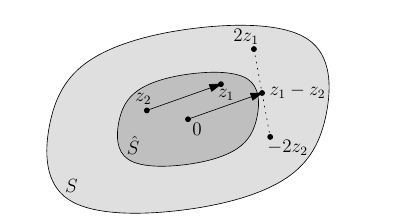
\includegraphics[scale=0.3]{minkowski-convex-body.png}
\end{center}
\end{frame}


\begin{frame}
\frametitle{Lattices}

The convex body theorem plus a lower bound on the volume of an $n-dimensional ball$ gives you an upper bound on the shortest vector.

This is given by \textbf{Minkowki's first theorem}: Every lattice $L$ contains a nonzero vector $v$ that satisfies 

\[ \norm{v} \leq \sqrt{n} (det(L)^{\frac{1}{n}}) \]

Which now gives us an interesting bound above and below for our shortest vector!

We can define also the \textbf{Hadamard Ratio} as:

\[ \mathcal{H}(B) = \bigg( \frac{det L}{\norm{v1}...\norm{v_n}} \bigg)^{\frac{1}{n}} \]

Where $0 < \mathcal{H}(B) \leq 1$ where the closer that value is to 1, the more orthogonal the vector is.

\end{frame}

\begin{frame}
\frametitle{GGH}

With bounds on our problem, we can start trying to look at a way we can contruct a lattice-based cryptosystem.

To start, we can notice that solving the SVP and CVP is incredibly easy for for a lattice $L$ with an orthogonal basis, since orthogonality degrades the euclidean norm of every single linear combination of the basis vectors to

\[ \norm{v} = \sum_{i \leq n} a_i^2 \norm{v_i}^2 \]

A similar thing happens when we have an orthogonal basis to try and solve the CVP.

\end{frame}

\begin{frame}
\frametitle{GGH}


The euclidean norm for some two vectors $w \in \rat^n, v \in L$ is also expressed as a single sum, except with a difference of coefficients, for $a_i \in \zee$ and $b_i \in \rat$:

\[ \norm{w-v} = \sum_{i \leq n} (a_i - b_i)^2 \norm{v_i}^2  \]

Since $a_i$ are integers, the easiest way to minimize the coefficient is simply take the closest integer to each $b_i$.

\end{frame}

\begin{frame}
\frametitle{GGH}
It's tempting to attempt to use this same method on any arbitrary basis, but the basis of the lattice needs to be at least close to orthogonality for this to work.

Recall how we proved earlier that the element of a lattice $L$ combined with it's fundamental parallelepiped form a partition of $\rat^n$. This means that to solve the CVP, we can attempt to approximate it via the unique decomposition into its corresponding partition, then finding the closest vertex of the Parallelepiped to $w$. This is fairly easy if you hvae the vector that translates $w$ into the lattice quadrant, and thus comes babai's algorithm:



\end{frame}

\begin{frame}
\frametitle{GGH}

\begin{center}
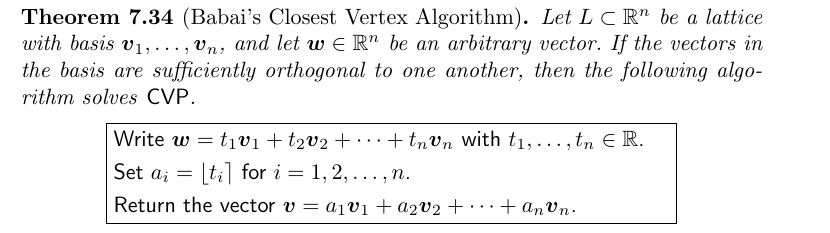
\includegraphics[scale=0.4]{babai.png}
\end{center}

\end{frame}

\begin{frame}
\frametitle{GGH}

With this, we can make our first cryptographic construction (Discovered by Goldreich, Goldwasser and Halevi):

Begin choosing a "Good" set of linearly independent vectors $v_1,...,v_n \in \zee^n$ that are reasonably orthogonal (check with Hadamard). This set is alice's private key, and we can denote the (Column-wise) matrix that this set spans by $V$. Then, pick a unimodular matrix $U$ such that you hvae $W = UV$ (U can be randomly chosen elementary matrices). The column vectors for $W$ are her public key.

\end{frame}

\begin{frame}
\frametitle{GGH}

When Bob wants to send us a message, he chooses a plaintext $m$ in the form of a vector (could be a binary vector), and small random perturbation vector $r$ (think of a nonce, but vector-style!).

To Encrypt, bob computes:

\[ e = Wm + r = \sum_{i-1}^n m_iw_i + r \]

Which is his ciphertext. For us to decrypt it, we use babai's algorithm combined with the "Good" basis we chose to find the smallest vector in $L$ close to $e$. Using the good basis with a small $r$ means we recover $Wm$, which we can multiply with $W^{-1}$ to recover $m$.

Unfortunately, GGH was proven impractical via Lattice reduction algorithms, which we will get to.


\end{frame}

\begin{frame}
\frametitle{NTRU}

The next cryptosystem we will toy with when it comes to lattices requires a bit more algebra to understand.

Let us define the \textit{ring of convolution polynomials} of rank $n$ as the quotient ring 

\[ R = \frac{\zee[x]}{x^n-1} \]

You can also have The ring of convolution polynomials over some modulus, by simply using:

\[ R_q = \frac{\zee_q[x]}{x^n-1} \] 


\end{frame}

\begin{frame}
\frametitle{NTRU}

Without spending too much time on this, we only need a few properties:
\begin{itemize}
\item The product of two polynomials in a convolution ring has its coefficients defined, for two polynomials in the ring $a(x)$ and $b(x)$ as \\
\[ c_k = \sum_{i+j \equiv k (mod n)} a_i b_{k-i}\] \\
Example: $a(x) = 1 - 2x + x^2$ and $b(x) = 3 - 5x$ with R of rank 3
\item Let $a(x) \in R_q$, the \textbf{center-lift} of $a(x)$ to $R$ is a unique polynomial $a'(x)$ such that $a'(x) mod q$ = $a(x)$, with coefficients $a_i \in (-\frac{q}{2}, \frac{q}{2}]$	
\item if $q$ is prime, then $a(x)$ in $R_q$ has a multiplicative inverse iff it is relatively prime to $x^n-1$.
\end{itemize}
\end{frame}

\begin{frame}
\frametitle{NTRU}

\textbf{\textit{Onto NTRUEncrypt:}}

\vspace{1em}

Fix the rank of your convolution polynomial ring to some prime $n$ and pick two relatively prime moduli $p$ and $q$ so you have $R$, $R_p$ and $R_q$, that also obey $gcd(n, q)= gcd(p, q) = 1$.

\vspace{1em}


We can observe a polynomial in the different rings using center-lifts (or in $R$ to $R_p$ or$R_q$, by taking the modulus).

\vspace{1em}


We also define a $T(d_1, d_2)$ as the function that categorizes the set of all ternary polynomials with $d_1$ coefficients set to $1$, and $d_2$ to $-1$, and the rest 0.

\end{frame}

\begin{frame}
\frametitle{NTRU}

Alice picks some $(n, p, q, d)$ with the constraints outlined above, and $q > (6d + 1) p$. She generates the private key consisting of two ternary polynomials $f(x) \in T(d+1, d)$ and $g(x) \in T(d, d)$. 

\vspace{1em}

Alice computes the inverses of $f(x)$: $F_q(x) \in R_q, F_p(x) \in R_p$, then computes $h(x) = F_q(x)g(x)$.  The pair $(f(x), F_p(x))$ is alice's private key. $h(x)$ is alice's public key.

\vspace{1em}


Bob sends a message to alice in the form of the coefficients of some polynomial $m(x)$ that satisfy $-\frac{1}{2}p < m_i \leq \frac{1}{2}p$ (meaning it's the center lift of another polynomial in $R_p$). Bob chooses a random polynomial $r(x) \in T(d, d)$ and computes 

\[ e(x) = p(h(x)r(x)) + m(x) \pmod{q} \]

Which makes $e(x)$ bob's ciphertext, in $R_q$.


\end{frame}

\begin{frame}
\frametitle{NTRU}

Alice decrypts $e(x)$ via the computations:
\begin{align*}
a(x) &= f(x)e(x)\pmod q \\
& \\
b(x) &= F_p(x)a(x)\pmod p
\end{align*}

We can prove rather easily, algebraically, that $b(x)$ and $m(x)$ match up, what is left is to prove that the coefficient bounds on our congruences makes $b(x)$ and $m(x)$ have the same coefficients.
	
\end{frame}

\begin{frame}
\frametitle{NTRU}

Alice decrypts $e(x)$ via the computations:
\begin{align*}
a(x) &= f(x)e(x)\pmod q \\
& \\
b(x) &= F_p(x)a(x)\pmod p
\end{align*}

We can prove rather easily, algebraically, that $b(x)$ and $m(x)$ match up, what is left is to prove that the coefficient bounds on our congruences makes $b(x)$ and $m(x)$ have the same coefficients.
	
\end{frame}

\begin{frame}
\frametitle{NTRU}

\begin{center}
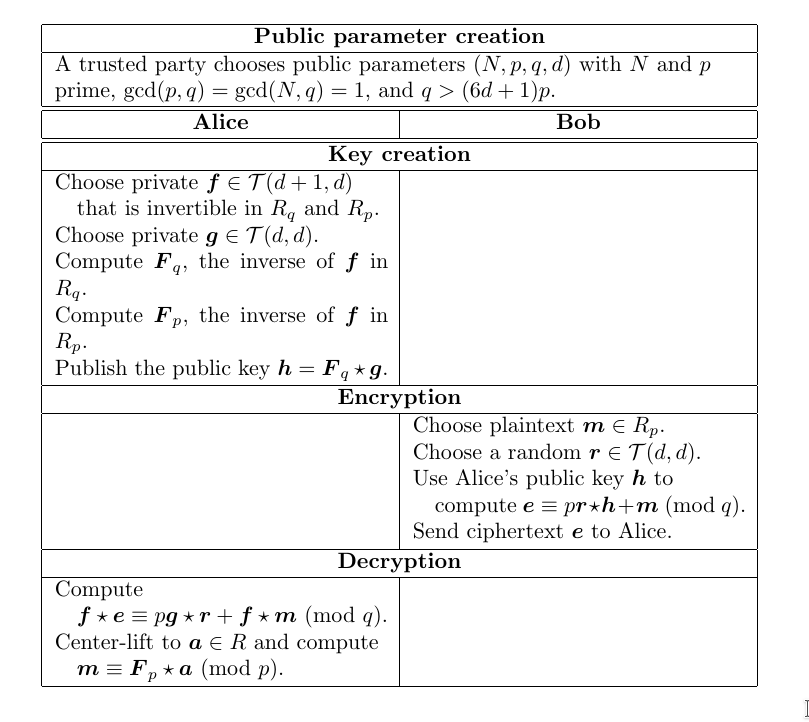
\includegraphics[scale=0.3]{Ntru-algo.png}
\end{center}

\end{frame}


\begin{frame}
\frametitle{NTRU}

Recall $h(x)$ (The public key) from our previous slide, and recall the polynomial coefficients look quite similar to a vector, with:

\[ h(x) = h_0 + h_1x +..+h_nx^n \]

The NTRU Lattice $L_h^{NTRU}$ is the $2n$-dimensional associated to $h(x)$ by:

\begin{center}
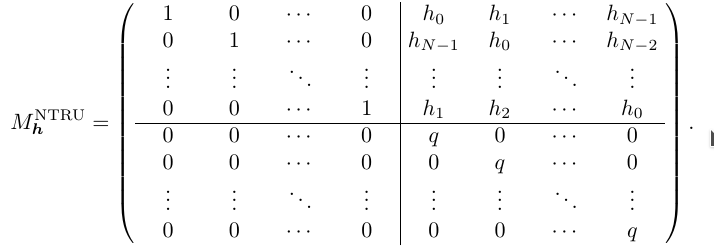
\includegraphics[scale=0.4]{Ntru-lattice.png}

\end{center}

\end{frame}

\begin{frame}
\frametitle{NTRU}

$M_h^{NTRU}$ is composed of:
\begin{enumerate}
\item left upper quadrant as the identity matrix
\item left lower quadrant sa the zero matrix
\item right lower quadrant as qI
\item right upper quadrant as the cyclical permutations (think the rotation) of the coefficients of $h(x)$.
\end{enumerate}

Often abbreviated as:

\[ M_h^{NTRU} = \begin{bmatrix}
I & h \\
0 & qI
\end{bmatrix} \]

\end{frame}
	
\begin{frame}
\frametitle{NTRU}
To try and convince ourselves that NTRUEncrypt truly is a lattice problem, we must show that the polynomial operations truly are lattice operations.

This is where the\textbf{ NTRUEncrypt Key recovery problem} appears. Despite the coefficients of some $h(x)$ appearing to be random (due to heuristic random distributions over modulus)	, there is a relationship:

\[ f(x)h(x) \equiv g(x) \pmod{q} \]

Where breaking NTRUEncrypt comes down to solving this congruence.

(Note: the relationship is not unique, due to cyclic rotations).

\end{frame}
	
\begin{frame}
\frametitle{NTRU}
With this in mind, the relationship can be stated equivalently as:

\[ f(x)h(x) \equiv g(x) + q(u(x)) \]

For some $u(x)$ satisfting that equality.

We can then perform the matrix multiplication:

\[ (f, -u) \begin{bmatrix}
I & h \\
0 & qI
\end{bmatrix} = (f, hf - qu) = (f, g)\]


\end{frame}

\begin{frame}
\frametitle{LLL (BONUS)}
\begin{center}
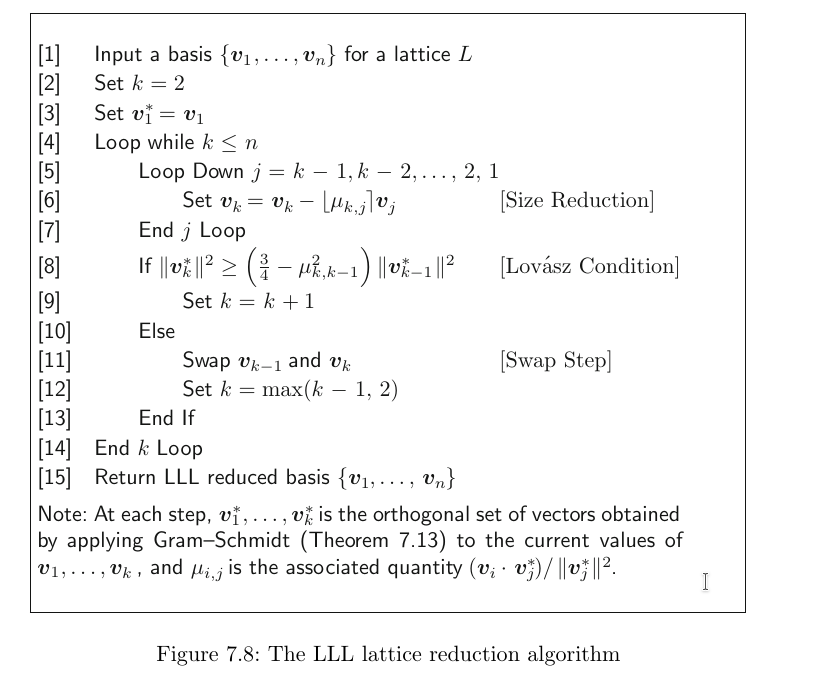
\includegraphics[scale=0.3	]{LLL-Reduction.png}
\end{center}


\end{frame}
	
\begin{frame}

Thank you!

References and further reading:

\begin{itemize}
\item Lecture notes by Dr. Chris Peikert for a graduate course on this topic (http://web.eecs.umich.edu/~cpeikert/lic15/index.html).
\item Lecture notes by the father of LWE, Dr. Oded Regev, in 2009: (https://cims.nyu.edu/~regev/teaching/lattices_fall_2009/index.html)
\item The book by Dr. Shari Goldwasser and Dr. Daniele Micciancio, \textit{Complexity of Lattice Problems, A Cryptographic Perspective}
\item CSC2414 Notes taught by Dr. Vinod Vaikuntanathan (MIT).
\item Abstract Algebra (Artin).
\item UTM Book: An Introduction to Mathematical Cryptography (Undergraduate Texts in Mathematics), by Hoffstein, Pipher and Silverman.
\end{itemize}

\end{frame}

\end{document}
